\chapter{GUI}
\begin{center}
   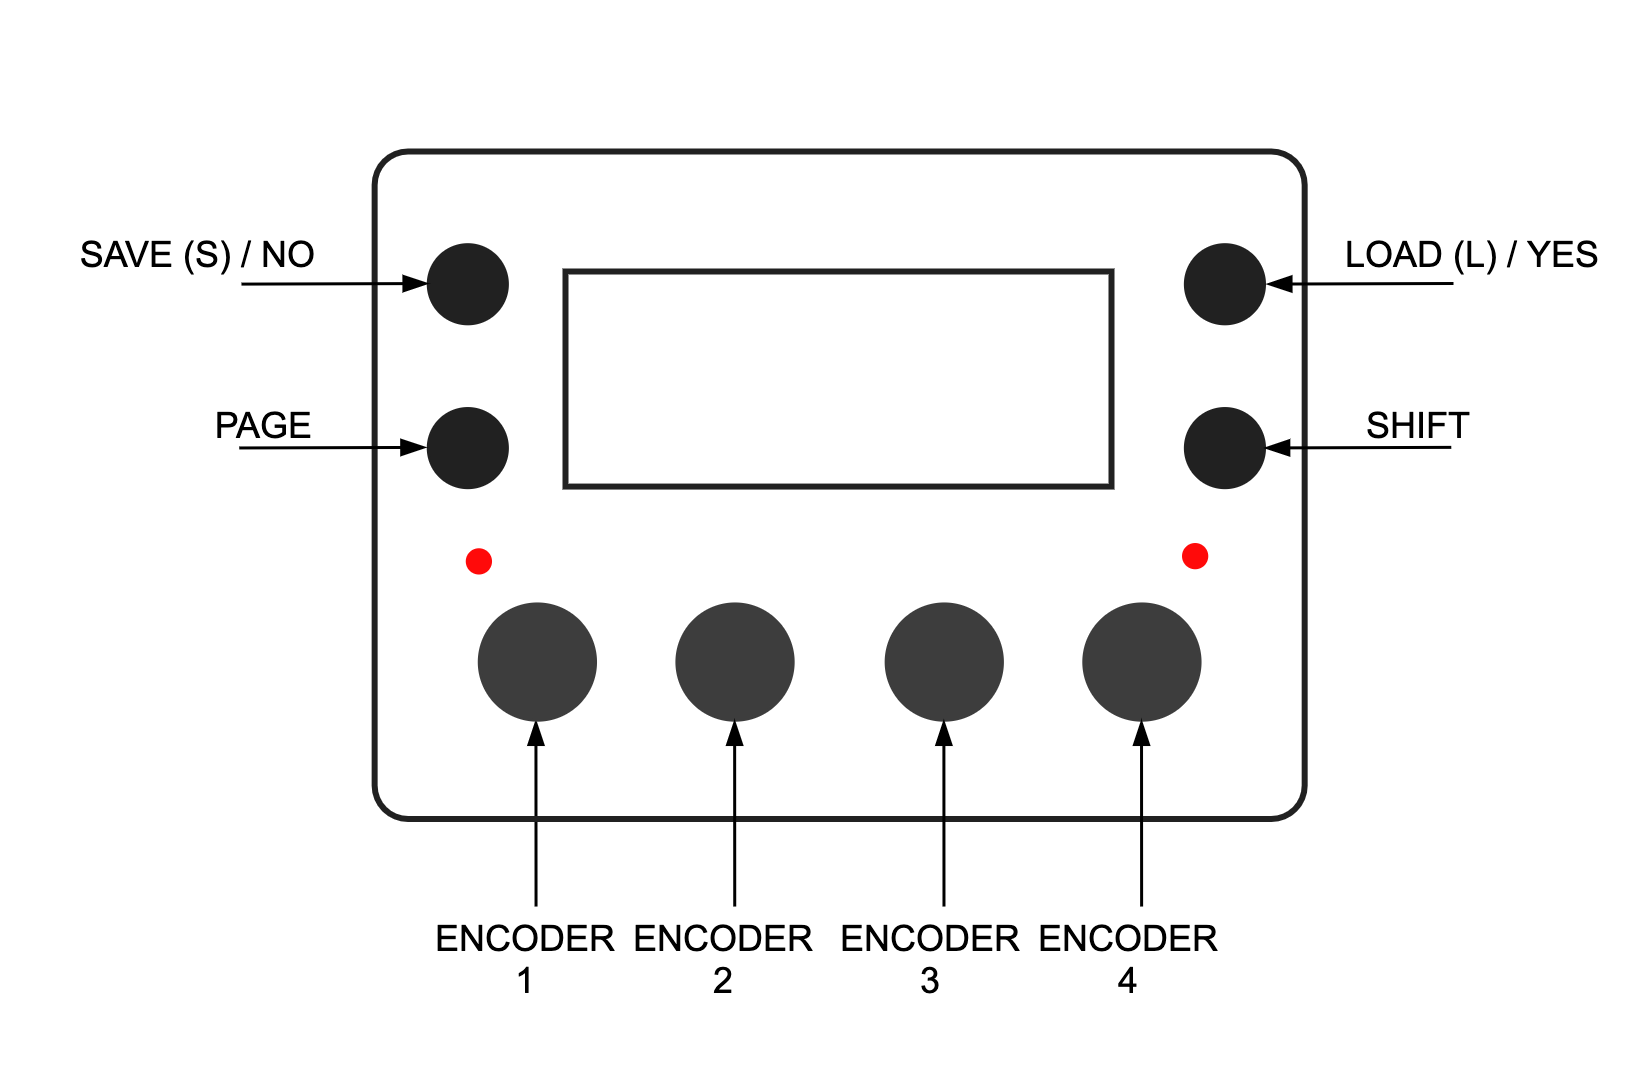
\includegraphics[width=18cm]{megacommand_gui.png}
\end{center}
\section{Function Buttons:}
From the Grid Page the function buttons perform the following actions:
\begin{itemize}
\item{\textbf{<Save | No>}: Enters the Save Page.}
\item{\textbf{<Load | Yes>}: Enters the Load page.}
\item{\textbf{<Page>}: Enters the PageSelect page.}
\item{\textbf{<Shift | Menu>}: Opens the slot Menu. }
\end{itemize}
Combined Button Presses:
\begin{itemize}
\item{\textbf{<Save | No> + <Load | Yes>}: Opens the MCL Configuration menu. }
\end{itemize}

\section{Encoder Buttons}
Encoder buttons are used to increase the speed of parameter rotation.
Holding down an encoder button whilst rotating the encoder will increase the update speed by 4x.

\newpage
\section{Machinedrum GUI: Enhanced Mode}
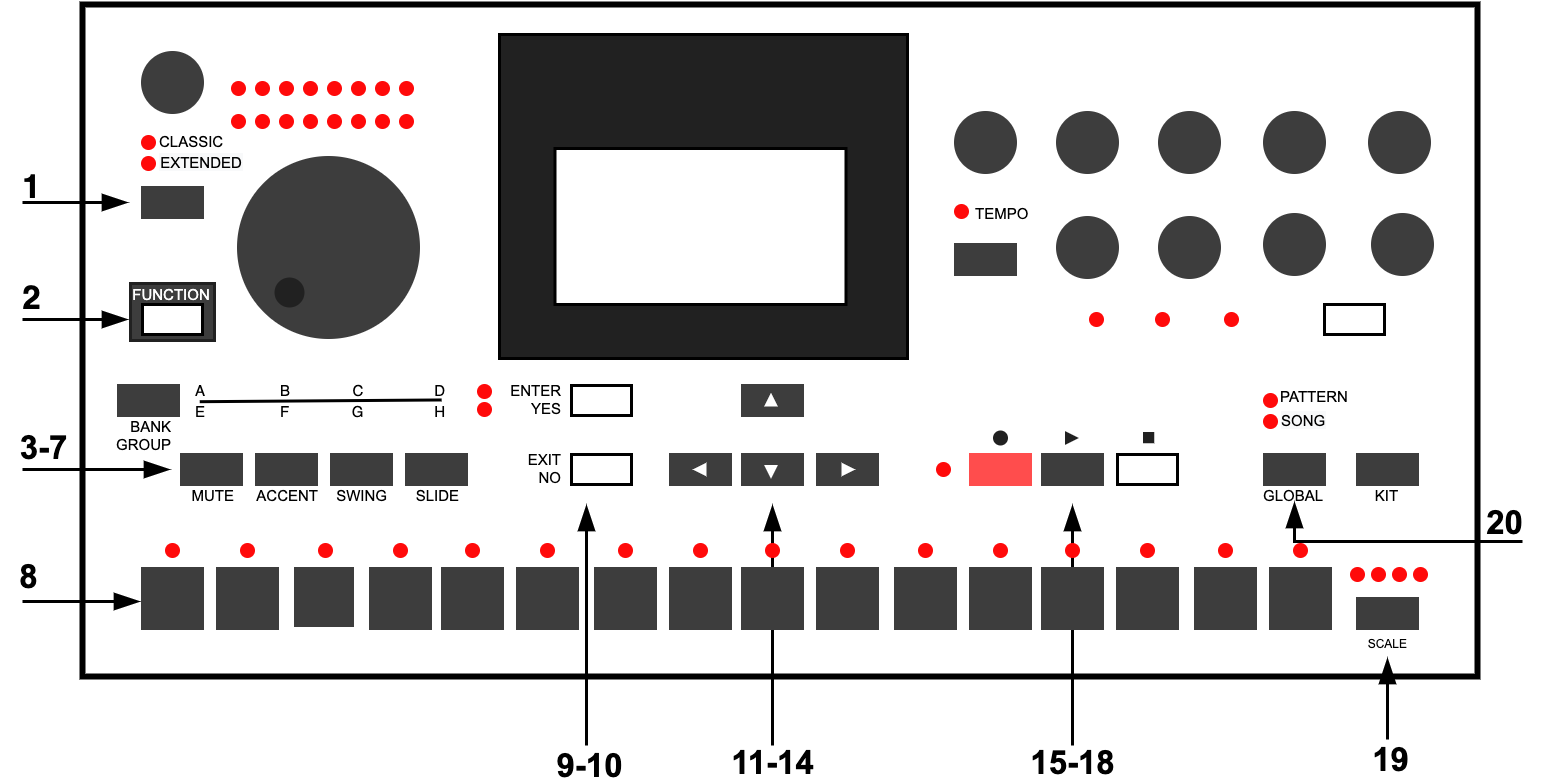
\includegraphics[width=18cm]{machinedrum_gui.png}

Version X.05 of the MD firmware introduces a third editing mode beyond Classic and Extended termed \textbf{Enhanced Mode}.\\
\\
Enhanced mode is activated automatically when the MD is connected to the MegaCommand.\\
\\
When in Enhanced mode, both Classic and Extended LEDs will be lit. The three modes can be toggled using the Classic/Extended button.\\
\\
Enhanced mode disable access to the MD's internal sequencer and enables the Machinedrum's GUI to be fully integrated with MCL as described on the next page.
\\
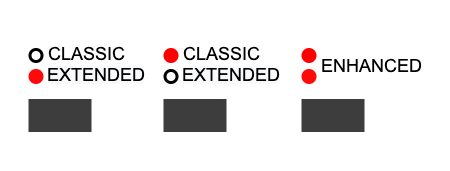
\includegraphics[width=10cm]{enhanced_mode.png}
\newpage
\section{MD + MCL command summary}
\begin{itemize}
\item \textbf{General:}
   \begin{itemize}
      \item \textbf{[Classic/Extended] } toggle between Classic, Extended and Enhanced Modes.
      \item \textbf{[Global] + [Trig] } page select.
      \item \textbf{[Bank] + [Trig]} loads slots from the selected row according to Group selection.
      \item \textbf{[Bank] + [Multiple Trigs]} creates a chain of slots from selected rows according to Group selection.
   \end{itemize}

\item \textbf{Grid Page:}
    \begin{itemize}
      \item \textbf{[Up/Down/Left/Right]} move grid cursor.
      \item \textbf{[Bank]} move grid cursor to start of bank.
      \item \textbf{[Clear/Copy/Paste]} all MD tracks.
      \item \textbf{[Function] + [Scale]} Opens the scale menu to set length and speed settings of all MD tracks.
      \item Hold \textbf{[No]} key to open Slot Menu.
      \begin{itemize}
                \item \textbf{[Bank]} keys can be used to select load mode: Manual, Auto or Queue.
                \item \textbf{[Up/Down/Left/Right]} to select multiple slots in the grid.
                \item \textbf{[Clear/Copy/Paste]} to clear/copy/paste selected slot(s).
                \item \textbf{[Yes]} load selected slots. Slots are loaded according to the current load MODE setting. If more than one row is selected, the MODE is automatically set to QUE, and the loaded slots are added to each column's playback queue.                
      \end{itemize}

\item \textbf{[Yes]} opens \textbf{Load Page:}
    \begin{itemize}
    \item Hold \textbf{[Yes]} to open slot Group Select. Release \textbf{[Yes]} to load groups. Groups selection editable via \textbf{[Trig]} keys 1-4.
    \item \textbf{[Trig]} keys are used to select and load sequencer tracks from slots of the current row.
    \item \textbf{[Bank]} keys can be used to quickly select the load mode: Manual, Auto or Queue.
    \end{itemize}
    
\item \textbf{[Func] + [Yes]} opens \textbf{Save Page:}
    \begin{itemize}
    \item Hold \textbf{[Yes]} to open slot Group Select. Release \textbf{[Yes]} to save groups.  Groups selection editable via \textbf{[Trig]} keys 1-4.
    \item \textbf{[Trig]} keys are used to select and save sequencer tracks to slots of the current row.
    \item \textbf{[Bank]} keys can be used to quickly select the save mode: Save, Merge or Import.
    \end{itemize}
\end{itemize}

\item \textbf{Mixer Page:}
      \begin{itemize}
       \item \textbf{[Trigs] + [MD Encoder]} simultaneously modify parameters across selected tracks. 
      \item \textbf{[No] + [Trig]} revert parameter for selected track.
       \end{itemize}
\newpage
\item \textbf{Chromatic Page:}
      \begin{itemize}
      \item \textbf{[Up/Down]} change octave
      \item \textbf{[Left/Right]} transpose
      \end{itemize}

\item \textbf{Sequencer:}
\begin{itemize}
      \item \textbf{[Record]} key to enter/exit MCL step editing.
      \item \textbf{[Record] + [Play]} to enter realtime record mode (on any page).
      \item \textbf{[Clear/Copy/Paste]} Clear/Copy/Paste for Track/Page/Step.
      \item \textbf{[Step] + [Left/Right]} Microtiming.
      \item \textbf{[Step] + [Up/Down]} Conditional.
      \item \textbf{[Function] + [Left/Right]} Shift track.
      \item \textbf{[Function] + [Up]} Reverse track.
      \item \textbf{[Function] + [Scale]} Opens the scale menu to set length and speed settings of the current MD track.
      \item \textbf{[Function] + [Bank B]} Edit Lock toggle
      \item \textbf{[Function] + [Bank C]} Edit Mute toggle
      \item \textbf{[Function] + [Bank D]} Edit Slide toggle
\end{itemize}
\end{itemize}



